\chapter{Planowanie misji}\label{ch:planowanie}

\begin{sekcja}{Misja zaczyna się od celu}
Planowanie zaczyna się kilka miesięcy przed lotem, gdy zespół ustala cel misji. Potem zespół badawczy projektuje, buduje i testuje eksperyment. Lot jest zwieńczeniem tych przygotowań.

Na początku zapisz w karcie misji (formularz F0):
\begin{itemize}
  \item cel misji: naukowy, techniczny albo szkoleniowy,
  \item wymagania ładunku: wysokość, czas w stratosferze, temperatura, orientacja, odzyskanie próbek,
  \item zespół i role (formularz F1),
  \item wstępny termin i miejsce startu.
\end{itemize}

\begin{wskazowka}Dla nowego zespołu najlepszy cel to lot szkoleniowy z prostym ładunkiem (kamera, rejestrator). Zespół uczy się procedur bez presji wyniku naukowego.\end{wskazowka}
\end{sekcja}

\begin{sekcja}{Interfejs z ładunkiem badawczym}
Platforma używa standardowych pudełek styropianowych w rozmiarze typu eurobox. To upraszcza współpracę z zespołem badawczym:
\begin{itemize}
  \item ładunek musi zmieścić się w pudełku i w limicie masy -- platforma tylko go podwiesza,
  \item pudełka łatwo się łączą (wypustki, pasy), więc montaż jest szybki,
  \item zespół badawczy pracuje niezależnie od zespołu platformy.
\end{itemize}

Zespół badawczy dostarcza przed misją:
\begin{itemize}
  \item masę i wymiary (z pudełkiem),
  \item opis zasilania -- ładunek ma własne baterie, platforma nie zasila ładunków,
  \item częstotliwości radiowe, które ładunek emituje (ryzyko zakłóceń z trackerem),
  \item wymagania: wysokość, temperatura, orientacja, czas,
  \item procedurę włączenia przed startem i wyłączenia po odzyskaniu.
\end{itemize}

\begin{uwaga}Ładunek badawczy przechodzi te same testy bezpieczeństwa i zgodności co platforma (sekcja~\ref{sec:testy}). Ładunek bez testów nie leci.\end{uwaga}
\end{sekcja}

\begin{sekcja}{Harmonogram}
Rysunek~\ref{fig:harmonogram} pokazuje typowy harmonogram. Najdłuższe etapy to budowa i testy eksperymentu. Formalności zaczynają się co najmniej 4 tygodnie przed lotem.

\begin{center}\resizebox{\linewidth}{!}{\rysHarmonogram}\end{center}
\captionof{figure}{Typowy harmonogram misji. T0 -- dzień startu.}\label{fig:harmonogram}
\end{sekcja}

\begin{sekcja}{Budżet masy}
Projektuj zestaw jako balon \textbf{lekki} (rozdział~\ref{ch:prawo}):
\begin{itemize}
  \item łączna masa ładunku (wszystko pod powłoką) poniżej \SI{4}{kg},
  \item masa każdego pakietu poniżej \SI{2}{kg},
  \item linka podwieszenia zrywa się przy sile poniżej \SI{230}{N}.
\end{itemize}

Zważ każdy element. Używaj mas zmierzonych, nie szacowanych. Zostaw zapas co najmniej \SI{10}{\percent}.

\renewcommand{\arraystretch}{1.6}
\begin{tabularx}{\linewidth}{@{}|L|P{25mm}|P{25mm}|@{}}\hline
\textbf{Element} & \textbf{Masa plan [g]} & \textbf{Masa zmierzona [g]}\\\hline
Spadochron & & \\\hline
Olinowanie, krętlik, linki & & \\\hline
Gondola platformy (z bateriami) & & \\\hline
Gondola ładunku & & \\\hline
\textbf{Razem: masa ładunku do kalkulatora} & & \\\hline
Powłoka (z karty katalogowej) & & \\\hline
\end{tabularx}
\end{sekcja}

\begin{sekcja}{Prędkość wznoszenia i ilość gazu}
Ilość gazu decyduje o prędkości wznoszenia. Prędkość wznoszenia decyduje o wysokości pęknięcia, czasie lotu i odległości lądowania.

\textbf{Heurystyka:}
\begin{itemize}
  \item \textbf{Szybsze wznoszenie} (więcej gazu): balon szybciej i niżej pęka, bo startuje bardziej napełniony. Lot jest krótszy i ląduje bliżej.
  \item \textbf{Wolniejsze wznoszenie} (mniej gazu): lot jest wyższy i dłuższy, ale balon dłużej dryfuje z wiatrem i może „uciec” -- wylądować bardzo daleko.
  \item \textbf{\SI{5}{m/s} to bezpieczne minimum.} Balon szybko wznosi się nawet przy słabym wietrze i szybko mija wysokość budynków, drzew i linii energetycznych.
\end{itemize}

\begin{center}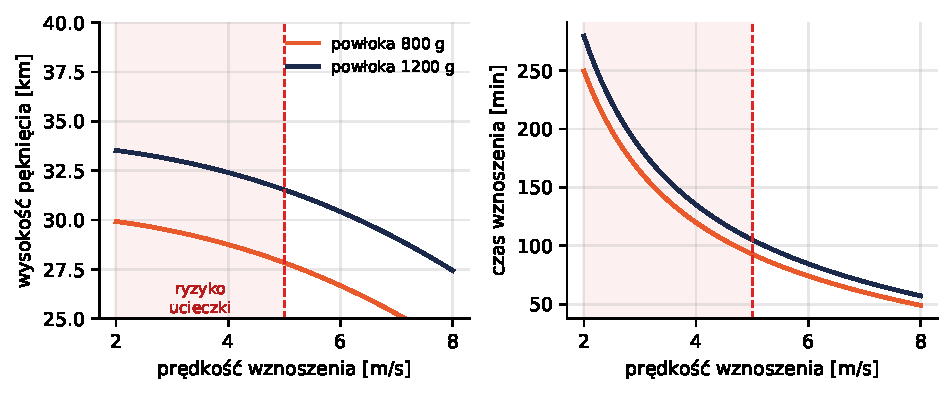
\includegraphics[width=\linewidth]{heurystyka_wznoszenia}\end{center}
\captionof{figure}{Wysokość pęknięcia i czas wznoszenia w funkcji prędkości wznoszenia. Obliczenia metodą kalkulatora SondeHub~\cite{sondehubcalc} dla ładunku \SI{2}{kg}. Obszar czerwony: ryzyko ucieczki.}\label{fig:heurystyka}
\end{sekcja}

\begin{sekcja}{Obliczenie ilości gazu}
\begin{enumerate}
  \item Zważ cały zestaw lotny bez powłoki.
  \item Otwórz kalkulator SondeHub: \url{https://sondehub.org/calc/}.
  \item Wpisz masę ładunku. Wybierz model powłoki.
  \item Wpisz docelową prędkość wznoszenia: \SI{5}{m/s}.
  \item Zapisz w karcie misji (F0): siłę nośną szyjki (\emph{neck lift}), objętość gazu, wysokość pęknięcia, czas do pęknięcia.
  \item Zamów gaz z zapasem co najmniej \SI{30}{\percent} (straty, powtórka, butla z mniejszą ilością gazu).
\end{enumerate}

\small
\begin{tabularx}{\linewidth}{@{}YYYYY@{}}
\toprule
\textbf{Wznoszenie [m/s]} & \textbf{Gaz [m³]} & \textbf{Siła nośna szyjki [kg]} & \textbf{Pęknięcie [km]} & \textbf{Wznoszenie [min]}\\\midrule
\wiersze{figures/generated/tabela_wznoszenia.tex}
\bottomrule
\end{tabularx}
\normalsize
\captionof{table}{Przykład: ładunek \SI{2}{kg}, powłoka \SI{800}{g} (średnica pęknięcia \SI{7}{m}). Tylko do orientacji -- dla swojej misji użyj kalkulatora.}
\end{sekcja}

\begin{sekcja}{Predykcja trajektorii}
\begin{enumerate}
  \item Otwórz predyktor SondeHub: \url{https://predict.sondehub.org/}.
  \item Wpisz miejsce startu, datę i godzinę, prędkość wznoszenia, wysokość pęknięcia i prędkość opadania.
  \item Sprawdź miejsce lądowania.
  \item Powtarzaj predykcję codziennie od około 7 dni przed lotem. Wpisuj wyniki do dziennika predykcji (formularz F4). Prognoza wiatru się zmienia.
  \item Wybierz termin i miejsce, dla których miejsce lądowania jest bezpieczne i dostępne.
\end{enumerate}
\end{sekcja}

\begin{sekcja}{Scenariusze zapasowe}
Po wysłaniu zgłoszenia do PAŻP nie możesz zmienić miejsca ani godziny startu. Dlatego:
\begin{itemize}
  \item wyślij \textbf{dwa zgłoszenia}: dla miejsca zasadniczego i dla miejsca zapasowego,
  \item w każdym zgłoszeniu podaj termin zasadniczy i termin zapasowy, np. 1--2 godziny po pierwszej godzinie albo inny dzień,
  \item przygotuj \textbf{plan działania dla każdego scenariusza}: kto jedzie gdzie, kiedy zespół decyduje, co robi, gdy żaden scenariusz nie jest bezpieczny.
\end{itemize}

\renewcommand{\arraystretch}{1.6}
\begin{tabularx}{\linewidth}{@{}|P{12mm}|L|L|L|@{}}\hline
\textbf{Scen.} & \textbf{Miejsce i godzina} & \textbf{Warunek wyboru} & \textbf{Plan działania}\\\hline
A & & & \\\hline
B & & & \\\hline
C & & & \\\hline
\end{tabularx}
\end{sekcja}

\begin{sekcja}{Kryteria braku startu}
\textbf{Nie startuj}, gdy predykcja pokazuje lądowanie:
\begin{itemize}
  \item w morzu, jeziorze albo na rozległym terenie podmokłym,
  \item w dużym lesie albo w mieście,
  \item w strefie kontrolowanej lotniska,
  \item za granicą państwa -- w szczególności w Rosji (obwód kaliningradzki), na Białorusi i na Ukrainie. Lot nad tymi państwami jest niedopuszczalny ze względu na sytuację geopolityczną. Odzyskanie ładunku jest tam niemożliwe, a lot może zostać uznany za incydent.
\end{itemize}

\textbf{Nie startuj}, gdy:
\begin{itemize}
  \item wiatr przy ziemi jest silny (tankowanie i start są niebezpieczne),
  \item pada deszcz, jest burza albo niska podstawa chmur,
  \item test trackera na stanowisku nie przeszedł (brak pozycji GPS albo brak odbioru telemetrii),
  \item którykolwiek punkt przeglądu gotowości (formularz F6) jest niespełniony.
\end{itemize}
\end{sekcja}

\begin{sekcja}{Wymagane testy}\label{sec:testy}
Wykonaj te testy przed każdą misją, dla platformy i dla każdego ładunku. Zapisz wyniki w formularzu F5.

\renewcommand{\arraystretch}{1.3}
\small
\begin{tabularx}{\linewidth}{@{}P{38mm}LP{30mm}@{}}
\toprule
\textbf{Test} & \textbf{Jak} & \textbf{Kryterium}\\\midrule
Funkcjonalny & Wszystkie funkcje na stole, z zasilania bateryjnego. & Wszystko działa.\\
W zimnie & Zamrażarka (\SI{-20}{\degreeCelsius}) albo zamrażarka laboratoryjna (\SI{-80}{\degreeCelsius}) przez czas lotu, urządzenia włączone. & Działa, zapisuje dane.\\
Zasięg radia & Tracker z anteną lotną; odbiór z odległości co najmniej \SI{100}{m}, najlepiej kilku km. & Pakiety odebrane, pozycja na mapie.\\
Odcinacz & Zwolnienie pod pełnym obciążeniem, ze skręconymi linkami, po schłodzeniu. & 10 z 10 prób.\\
Czas pracy & Cały system na bateriach lotnych. & $\geq 2\times$ czas lotu + czas poszukiwań.\\
Upadek & Gondola zrzucona z około \SI{1}{m} na twarde podłoże. & Nic się nie odłącza.\\
Próba generalna & Cały montaż i formularze dnia startu, bez balonu. & Zespół zna role i kolejność.\\
\bottomrule
\end{tabularx}
\normalsize

\begin{wskazowka}Zapytaj biologów na Wydziale Chemicznym, czy możesz użyć ich zamrażarki laboratoryjnej. Zamrażarki do przechowywania próbek osiągają \SI{-80}{\degreeCelsius} -- warunki bliższe stratosferze niż domowa zamrażarka.\end{wskazowka}
\end{sekcja}

\begin{sekcja}{Przegląd gotowości do startu}
Kilka dni przed lotem zespół robi przegląd gotowości (\emph{Flight Readiness Review}). Kierownik misji przechodzi z zespołem przez formularz F6. Każdy punkt ma dowód: wynik testu, potwierdzenie z PAŻP, zdjęcie, wpis w karcie misji.

Wynik przeglądu to decyzja „leci / nie leci”. Brak dowodu oznacza „nie leci”, dopóki zespół go nie dostarczy.
\end{sekcja}
